\chapter{The Data}
\label{cha:data}
As Markus Schmitt states in \cite{Schmitt2018} that the data is one of the most important if not the most important
factor in a machine learning project, for this reason we will take a deeper look into our data.
In the following chapter we present
the LRS3 dataset (described in Section \ref{sec:lrs3}) we use to construct the VVAD dataset (described in Section \ref{sec:vvadData}).
How we extract positive and negative samples from it is described in Section \ref{ssec:dataAcquisition}.
Section \ref{ssec:dataPreprocessing} covers the necessary steps in the preprocessing.
In general one has to distinguish between the training data and the test data. While the training data is
used to train the chosen machine learning algorithm, the test data is used to evaluate how good the algorithm performs.
The construction of the test set is described in Section \ref{ssec:testset}.
A general description what data needs to fulfill in order to be learnable and how to split data into training, validation and test set is given in Section \ref{ssec:dataTheory}
The results and how the evaluation is performed is presented in Chapter \ref{cha:eval}.

\section{Lip Reading Sentences 3 (LRS3) Dataset}\label{sec:lrs3}
Since the VVAD is implemented with a learning algorithm, to reduce the false positive rate, which is relatively high in the classic approach of lip motion detection (see Section \ref{sec:relatedWorks}).
The learning algorithm should be able to distinguish between a natural lip motion in \emph{ not speaking} phases and the lip motion which is associated with \emph{speaking} phases.
To accomplish that a dataset with a large amount of natural \emph{speaking} and \emph{not speaking} scenarios is needed.
Triantafyllos Afouras et al. introduced in \cite{Chung18} a large-scale dataset for visual speech recognition from videos of 5594 TED and TEDx talks.
It provides more than 400 hours video material of natural speech.
Which is substantially more compared to other
public datasets that are available for general research.
A comparison of datasets is shown in figure \ref{fig:datasetCompare}.

\begin{figure}
  \centering
  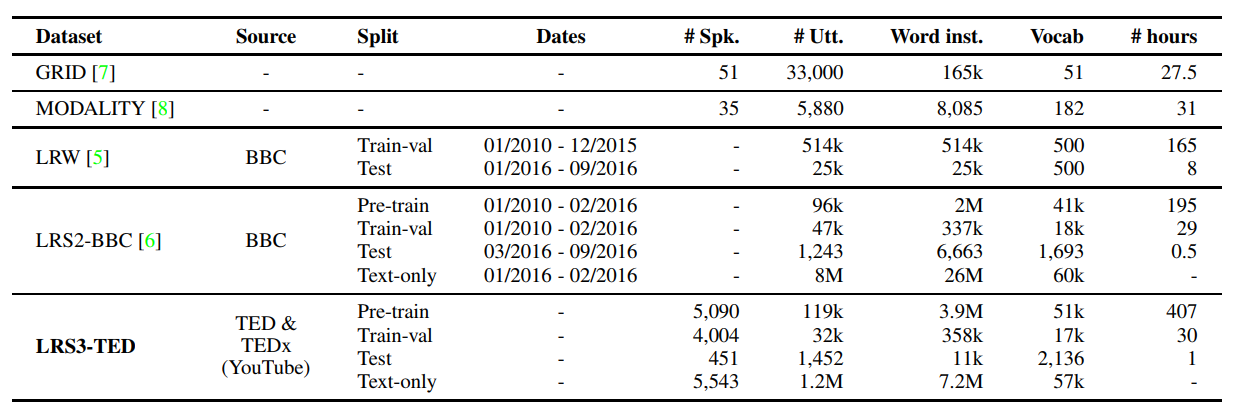
\includegraphics[width=.95\textwidth]{datasetCompare.png}
  \caption{A comparison of publicly available lip reading datasets. Division of training, validation and test data; and the number of utterances, number
of word instances and vocabulary size of each partition. Utt: Utterances.\cite{Chung18}}
  \label{fig:datasetCompare}
\end{figure}

The LRS3 dataset provides videos of TED and TEDx talks along with text files containing information about the position of the face and the said words.
In the text file the following fields are important for the transformation to the VVAD dataset (An example of a LRS3 sample can be found in Appendix \ref{app:dataSample}):
\paragraph{Text} contains the text for one sample. The length of the text or respectively the sample is defined by length of the scene. 
That means one sample can get as long as the face is present in the video.
\paragraph{Ref} is the reference to the corresponding YouTube video. The value of this field needs to be appended to \texttt{https://www.youtube.com/watch?v=}
\paragraph{FRAME} corresponds to the face bounding box for every frame, where \texttt{FRAME} is the frame number, \texttt{X} and \texttt{Y} is the position of the bounding box in the video and \texttt{W} and \texttt{H} are the width and height of the bounding box respectively. It is to mention that for the frame number a frame rate of 25 fps is assumed and the values for \texttt{X}, \texttt{Y}, \texttt{W} and \texttt{H} are a percentage indication of the width and height of the video.
\paragraph{WORD} maps a timing to every said word. Here \texttt{START} and \texttt{END} indicate the start and end of the word in seconds respectively. 
It is to mention that the time is in respect to the start of the sample given by the first frame and not to the start of the whole video.
\paragraph{}%Pseudo end

The LRS3 dataset comes with a very low bias towards specific ethnic groups, because TED and TEDx talks are international and talks are held by men and women as well as by kids. 
It also comes with the advantage that it depicts a huge variety of people because the likelihood of talking in multiple TED or TEDx talks is rather small.
This is a big advantage over the LRS2 and LRW dataset that are extracted from regular TV shows, which brings the risk of overfitting to a specific persons. 
LRS3 makes learning more robust in that sense. 
Since natural speech in front of an audience includes pauses for applause and means to structure and control a speech as described in \cite{Nikitina2011}, the LRS3 dataset provides \emph{speaking} and \emph{not speaking} phases.
How we extracted the positive (\emph{speaking}) and negative (\emph{not speaking}) samples from the LRS3 dataset is described in Section \ref{ssec:dataAcquisition}.


\section{VVAD Dataset}\label{sec:vvadData}
From the LRS3 dataset described in Section \ref{sec:lrs3} a new dataset is constructed.
The newly created dataset will be call VVAD dataset.
The close relation between lipreading and VVAD makes it possible to adjust the LRS3 to be used for the purpose of Visual Voice Activity Detection
The VVAD dataset is created by an automated process depicted in Section \ref{sec:createVVAD}.
The produced VVAD dataset comes in four different flavors for the samples.
These flavors are related to the four different learning approaches described in Section \ref{ssec:algorithm} and are visualized in Figure \ref{fig:flavors}.
\paragraph{Face Images} used for the most sophisticated model.
These Face Images come in a maximal resolution of $200 \times 200$ pixels and with a maximal number of 38 frames.
So the maximal shape of one sample of the flavor \emph{Face Images} is $38 frames \times 200 pixels \times 200 pixels \times 3 channels = 4560000$.
Face Images are RGB images, so the 3 channels correspond to the 3 RGB channels.
Pixel values range between 0 and 255 which can be represented with one byte. 
This means one \emph{Face Images} sample takes 4560000 bytes, which equals $4.56$ mega bytes.
\paragraph{Lip Images} are also used for an End-to-End learning approach but they obviously concentrate on a small subset of the Face Images.
As well as the Face Images, the Lip Images are RGB images coming with a maximum of 38 frames but they have a maximal resolution of $100 \times 50$ pixels.
This resolves to a size of $0.57$ mega bytes given by $38 frames \times 100 pixels \times 50 pixels \times 3 channels = 570000$
\paragraph{Face Features} are used for the learning approach which focuses on facial features. 
These facial features are landmarks extracted from dlib's facial landmark detector 
as described in Section \ref{sec:createVVAD}.
It provides 68 landmarks with a (X,Y)-Position for a single face as depicted in Figure 
\ref{fig:shape}.
A single feature is given as float64 (8 bytes), resulting in a size of $41.344$ kilo bytes, given by $38 frames \times 68 features \times 2 \times 8 bytes = 41344$.
\paragraph{Lip Features} are a small subset of Face Features that only take the features of the lips into account. 
Dlib's facial landmark detector
reserves 20 features for the lips as shown in Figure \ref{fig:shape}.
This results in the size of $38 frames \times 20 features \times 2 \times 8 bytes = 12160$ for a single sample in the lip features flavor.

\begin{figure}
\centering
\parbox{\textwidth}{
\begin{subfigure}{.5\textwidth}
  \centering
  \captionsetup{width=.8\linewidth}
  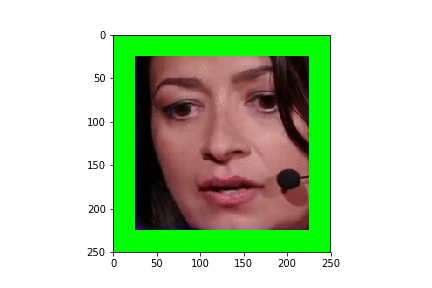
\includegraphics[width=\linewidth]{faceImages.png}
  \caption{Visualization of one frame in \emph{Face Images} flavor}
\end{subfigure}%
\begin{subfigure}{.5\textwidth}
  \centering
  \captionsetup{width=.8\linewidth}
  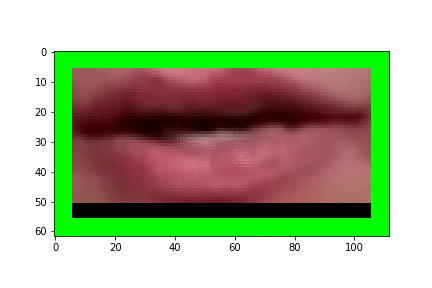
\includegraphics[width=\linewidth]{lipImages.png}
  \caption{Visualization of one frame in \emph{Lip Images} flavor}
\end{subfigure}
}
\parbox{\textwidth}{
\begin{subfigure}{.5\textwidth}
  \centering
  \captionsetup{width=.8\linewidth}
  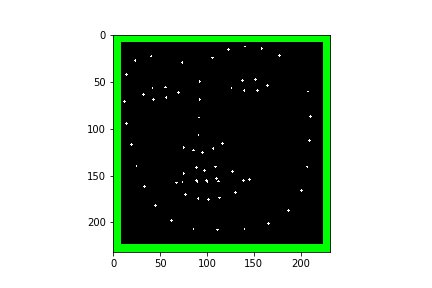
\includegraphics[width=\linewidth]{faceFeatures.png}
  \caption{Visualization of one frame in \emph{Face Features} flavor}
\end{subfigure}%
\begin{subfigure}{.5\textwidth}
  \centering
  \captionsetup{width=.8\linewidth}
  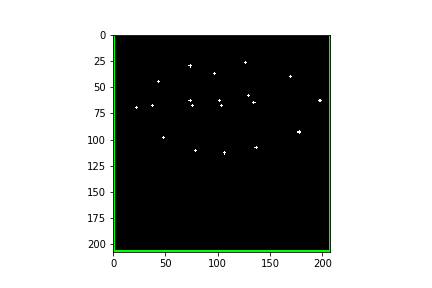
\includegraphics[width=\linewidth]{lipFeatures.png}
  \caption{Visualization of one frame in \emph{Lip Features} flavor}
\end{subfigure}%
}
\caption{Visualization for the different flavors.}
\label{fig:flavors}
\end{figure}

As the VVAD dataset is designed for binary classification it provides two classes.
The positive class in this case is \emph{speaking}, while the negative class is \emph{not speaking}. This holds for all the different flavors and takes one byte per sample.
The VVAD dataset comes with 44,289
samples equally distributed to the classes (22,144 
positive samples and 22,145 
negative samples) for training and validation set.
The total size of the VVAD dataset in bytes can be calculated with $(|S| + 1) \times |D|$, where $|S|$ is the size of one sample and $|D|$ the total number of samples in the dataset. 
The size of the sample is incremented by one because the label for every sample takes another byte.
This results in the following total sizes for the different flavors:
\begin{itemize}
\item[•] \textbf{Face Images:} $(4,560,000 + 1) bytes \times 44,289 = 201,957,884,289 bytes \approx 201.96 GB $ 
\item[•] \textbf{Lip Images:} $(570,000 + 1) bytes \times 44,289 = 25,244,774,289 bytes \approx 25.24 GB $ 
\item[•] \textbf{Face Features:} $(41,344 + 1) bytes \times 44,289 = 1,831,128,705 bytes \approx 1.83 GB $ 
\item[•] \textbf{Lip Features:} $(12,160 + 1) bytes \times 44,289 = 538,598,529 bytes \approx 538.6 MB $ 
\end{itemize}
Although it would be possible to construct a larger dataset it was chosen to create a balanced dataset.
This means all classes in the data are equally distributed.
An imbalanced dataset impose the danger of the learning algorithm taking shortcuts.
Imagining a very imbalanced binary dataset which has 90\% positive samples and 10\% negative samples.
The problem here is that learning is basically an optimization process, which aims to minimize a loss function.
If the loss function is just measuring how good the output matches the input over all samples it is obvious that the output will be optimized to show the positive class.
If the validation set has the same distribution as the training set this will give a accuracy of 90\%.
Which seems to be pretty good on first sight but if a closer look is taken the classifier unfolds to classifying everything as positive because it works for most of the samples.
There are techniques like undersampling, oversampling, synthetic data generation and cost sensitive learning to prevent this problem which will not be discussed any further because the easiest solution is to create a balanced dataset.
The creation of a balanced dataset is not always possible but as described in Section \ref{ssec:dataAnalysis} it is possible for the VVAD dataset.


\subsection{Test Set}\label{ssec:testset}
As described in Section \ref{ssec:VVADHACL} a human accuracy level test is performed on a small representative subset of 200 samples.
These 200 samples will be used as the test set to ensure the comparability between the results of the developed VVAD and the human accuracy level empirically determined by the human accuracy level test.
The test set contains the same samples for every flavor and can be used to verify the accuracy for the different learning approaches.




\section{Potential Problems with Big Data}\label{sec:problemsBigData}
The National Institute of Standards and Technology (NIST) defines Big Data the following: 
\begin{quote}
\textit{Big Data consists of extensive datasets - primarily in the characteristics of volume, variety, velocity, and/or
variability - that require a scalable architecture for efficient storage, manipulation, and analysis.}\cite{NIST2018}
\end{quote}
In general when we look at the complexity of an algorithm two aspects should be considered. The first aspect is the amount of processing time the algorithm needs. The other aspect is the amount of space or memory the algorithm needs. Memory is primary considered as RAM (Random-Access Memory) but when it comes to Big Data one also needs to consider the space a dataset takes on hard drive. 
If you don't have infinite time and space, which you never have, you want to optimize your algorithm in one direction or find a compromise between both aspects.

In relation to the datasets described in Section \ref{sec:lrs3}-\ref{sec:vvadData} and the data acquisition described in \ref{ssec:dataAcquisition} this leads to some potential problems, which will be discussed in the following.
On the hardware used to produce the VVAD dataset there is a 1.5 TB hard drive designated for data. 
The original downloaded LRS3 dataset takes approximately 500 GB, leaving 1 TB for datasets constructed via the proposed data acquisition. 
At this point the first problem arises: How to save the constructed dataset? 
As described in \ref{ssec:dataAcquisition} a sample consists out of \texttt{k} frames of features, which can of pixels or facial features extracted from an image and a positive or negative label. 
Space efficient would be to get the samples from the encoded videos every time they are needed for a training of the algorithm.
This is not an in-depth definition of encoding, but what it basically does is to save the difference between to frames, which is in a video very little, so it saves a lot of space but needs a little more time to calculate the next frame from the previous. On the other hand saving the raw frames is time efficient put costs more space.
So getting the sample directly from the video is space efficient because no extra space is needed to save the newly constructed samples.
But the following example shows that this is highly time inefficient.
Experiments have shown that it takes approximately 1143.856 s to get 100 samples from the videos, while it takes only 0.127 s to get 100 previously saved samples from the hard drive. This is more than 9000 times faster. Knowing 900 thousand samples can be produced from the LRS3 dataset it will take approximately 120 days to get all samples. With the hardware used to produce the VVAD dataset it is possible to parallelize the process in 12 cores. 
To implement this parallel processing of the videos the producer-consumer patterns was applied. 
12 producer run in parallel to produces samples from videos while one consumer saves these samples in a given ratio to the hard drive. This shrinks the time to produce a dataset to around 10 days. This is suitable for doing it once but not for every training considering there is a process of tuning the parameters, which takes multiple training sessions to complete. 
On the one hand it is obvious that it is not suitable to get the samples from the videos for every training, on the other hand the space this newly constructed dataset consumes needs to be determined.  
Assuming a sample with a \texttt{sampleLength} of 1.5 seconds and a shape of $200\times200$ pixels, the sample consumes approximately 4.5 MB. Figure \ref{fig:sampleDistribution} shows that with the given \texttt{sampleLength} a total number of over 900 thousand samples can be constructed. Applying that to the 4.5 MB, the constructed dataset will take approximately 4 TB. This space is not available on the hardware used to produce the VVAD dataset.
Here the first problem arises which needs to be solved implementing a compromise. 
The analysis of the data shows that for the purpose of the VVAD only a very imbalanced dataset can be constructed (see Figure \ref{fig:sampleDistribution}), knowing that it is possible to reduce the size needed by only saving a balanced dataset. 
This makes sense from a perspective of capacity, in Section \ref{sec:vvadData}
it is described why it makes sense to under-/oversample to a balanced dataset from a learning perspective.
Saving a dataset with a positive-to-negative-ratio of 1 to 1 instead of 30 to 1 needs approximately 266 GB.
